%%%%%%%%%%%%%%%%%%%%%%%%%%%%%%%%%%%%%%%%%%%%%%%%%%%%%%%%%%%%%%%%%%%%%%%%%%%
%% This file is part of the book
%%
%% Algorithmic Graph Theory
%% http://code.google.com/p/graph-theory-algorithms-book/
%%
%% Copyright (C) 2009, 2010, 2011 Minh Van Nguyen <nguyenminh2@gmail.com>
%%
%% See the file COPYING for copying conditions.
%%%%%%%%%%%%%%%%%%%%%%%%%%%%%%%%%%%%%%%%%%%%%%%%%%%%%%%%%%%%%%%%%%%%%%%%%%%

\documentclass{article}

\usepackage{subfigure}
\usepackage{tikz}
\usetikzlibrary{external}
\usetikzlibrary{shapes}
\usetikzlibrary{trees}
\tikzexternalize{AVL-trinode-restructure}

\begin{document}

\begin{figure}
\subfigure[Left rotation of $y$ over $z$.]{
\label{fig:tree_data_structures:AVL_trinode_restructure:single_left_rotate}
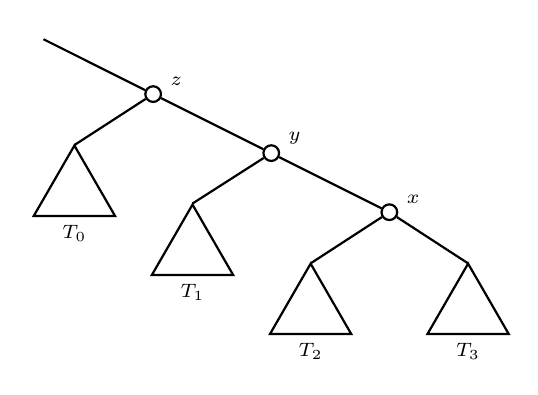
\begin{tikzpicture}
[-,thick,%
  lineDecorate/.style={-,thick},%
  nodeDecorate/.style={shape=regular polygon,regular polygon sides=3,inner sep=6pt,draw,thick},%
scale=0.5]
\scriptsize
%% nodes and edges
\node at (0,0) {}
  [sibling distance=6cm]
  child[missing]
  child {node[shape=circle,inner sep=2pt,draw] (z) {}
    child[missing]
    child {node[shape=circle,inner sep=2pt,draw] (y) {}
      child[missing]
      child {node[shape=circle,inner sep=2pt,draw] (x) {}}
    }
  };
%% node labels
\node[above right] at (z.east) {$z$};
\node[above right] at (y.east) {$y$};
\node[above right] at (x.east) {$x$};
%% generic trees and their labels
\foreach \nodename/\x/\y/\direction/\navigate in {
  T_0/1/-4/below/south, T_1/4/-5.5/below/south, T_2/7/-7/below/south,
  T_3/11/-7/below/south}
{
  \node[nodeDecorate] (\nodename) at (\x,\y) {};
  \node [\direction] at (\nodename.\navigate) {$\nodename$};
}
%% connect nodes to generic trees
\path
(z) edge[lineDecorate] node {} (1,-2.795)
(y) edge[lineDecorate] node {} (4,-4.28)
(x) edge[lineDecorate] node {} (7,-5.8)
(x) edge[lineDecorate] node {} (11,-5.8);
\end{tikzpicture}
%%
%%
\qquad\qquad
%%
%%
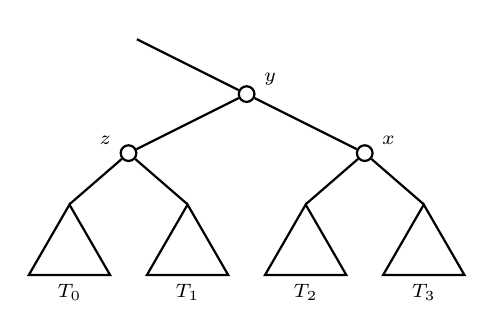
\begin{tikzpicture}
[-,thick,%
  lineDecorate/.style={-,thick},%
  nodeDecorate/.style={shape=regular polygon,regular polygon sides=3,inner sep=6pt,draw,thick},%
scale=0.5]
\scriptsize
%% nodes and edges
\node at (0,0) {}
  [sibling distance=6cm]
  child[missing]
  child {node[shape=circle,inner sep=2pt,draw] (y) {}
    child {node[shape=circle,inner sep=2pt,draw] (z) {}}
    child {node[shape=circle,inner sep=2pt,draw] (x) {}}
  };
%% node labels
\node[above left] at (z.west) {$z$};
\node[above right] at (y.east) {$y$};
\node[above right] at (x.east) {$x$};
%% generic trees and their labels
\foreach \nodename/\x/\y/\direction/\navigate in {
  T_0/-1.5/-5.5/below/south, T_1/1.5/-5.5/below/south,
  T_2/4.5/-5.5/below/south, T_3/7.5/-5.5/below/south}
{
  \node[nodeDecorate] (\nodename) at (\x,\y) {};
  \node [\direction] at (\nodename.\navigate) {$\nodename$};
}
%% connect nodes to generic trees
\path
(z) edge[lineDecorate] node {} (-1.5,-4.3)
(z) edge[lineDecorate] node {} (1.5,-4.3)
(x) edge[lineDecorate] node {} (4.5,-4.3)
(x) edge[lineDecorate] node {} (7.5,-4.3);
\end{tikzpicture}
}
%%
%%
\subfigure[Right rotation of $y$ over $z$.]{
\label{fig:tree_data_structures:AVL_trinode_restructure:single_right_rotate}
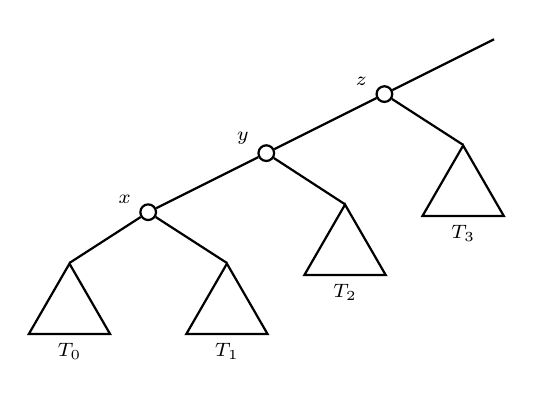
\begin{tikzpicture}
[-,thick,%
  lineDecorate/.style={-,thick},%
  nodeDecorate/.style={shape=regular polygon,regular polygon sides=3,inner sep=6pt,draw,thick},%
scale=0.5]
\scriptsize
%% nodes and edges
\node at (0,0) {}
  [sibling distance=6cm]
  child {node[shape=circle,inner sep=2pt,draw] (z) {}
    child {node[shape=circle,inner sep=2pt,draw] (y) {}
      child {node[shape=circle,inner sep=2pt,draw] (x) {}}
      child[missing]
    }
    child[missing]
  }
  child[missing];
%% node labels
\node[above left] at (z.west) {$z$};
\node[above left] at (y.west) {$y$};
\node[above left] at (x.west) {$x$};
%% generic trees and their labels
\foreach \nodename/\x/\y/\direction/\navigate in {
  T_0/-11/-7/below/south, T_1/-7/-7/below/south,
  T_2/-4/-5.5/below/south, T_3/-1/-4/below/south}
{
  \node[nodeDecorate] (\nodename) at (\x,\y) {};
  \node [\direction] at (\nodename.\navigate) {$\nodename$};
}
%% connect nodes to generic trees
\path
(z) edge[lineDecorate] node {} (-1,-2.79)
(y) edge[lineDecorate] node {} (-4,-4.3)
(x) edge[lineDecorate] node {} (-7,-5.79)
(x) edge[lineDecorate] node {} (-11,-5.79);
\end{tikzpicture}
%%
%%
\qquad\qquad
%%
%%
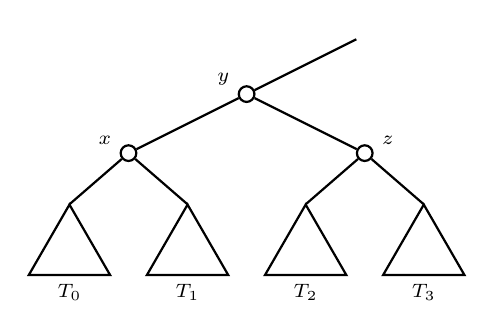
\begin{tikzpicture}
[-,thick,%
  lineDecorate/.style={-,thick},%
  nodeDecorate/.style={shape=regular polygon,regular polygon sides=3,inner sep=6pt,draw,thick},%
scale=0.5]
\scriptsize
%% nodes and edges
\node at (0,0) {}
  [sibling distance=6cm]
  child {node[shape=circle,inner sep=2pt,draw] (y) {}
    child {node[shape=circle,inner sep=2pt,draw] (x) {}}
    child {node[shape=circle,inner sep=2pt,draw] (z) {}}
  }
  child[missing];
%% node labels
\node[above right] at (z.east) {$z$};
\node[above left] at (y.west) {$y$};
\node[above left] at (x.west) {$x$};
%% generic trees and their labels
\foreach \nodename/\x/\y/\direction/\navigate in {
  T_0/-7.5/-5.5/below/south, T_1/-4.5/-5.5/below/south,
  T_2/-1.5/-5.5/below/south, T_3/1.5/-5.5/below/south}
{
  \node[nodeDecorate] (\nodename) at (\x,\y) {};
  \node [\direction] at (\nodename.\navigate) {$\nodename$};
}
%% connect nodes to generic trees
\path
(x) edge[lineDecorate] node {} (-7.5,-4.3)
(x) edge[lineDecorate] node {} (-4.5,-4.3)
(z) edge[lineDecorate] node {} (-1.5,-4.3)
(z) edge[lineDecorate] node {} (1.5,-4.3);
\end{tikzpicture}
}
%%
%%
\subfigure[Double rotation: right rotation of $x$ over $y$, then left
rotation over $z$.]{
\label{fig:tree_data_structures:AVL_trinode_restructure:right_left_rotate}
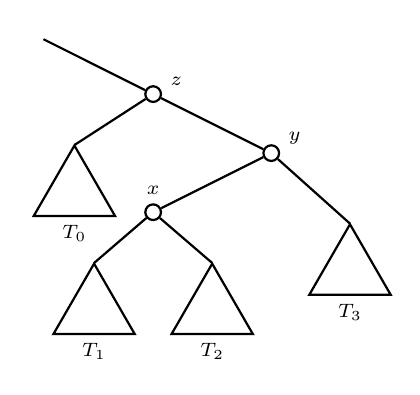
\begin{tikzpicture}
[-,thick,%
  lineDecorate/.style={-,thick},%
  nodeDecorate/.style={shape=regular polygon,regular polygon sides=3,inner sep=6pt,draw,thick},%
scale=0.5]
\scriptsize
%% nodes and edges
\node at (0,0) {}
  [sibling distance=6cm]
  child[missing]
  child {node[shape=circle,inner sep=2pt,draw] (z) {}
    child[missing]
    child {node[shape=circle,inner sep=2pt,draw] (y) {}
      child {node[shape=circle,inner sep=2pt,draw] (x) {}}
      child[missing]
    }
  };
%% node labels
\node[above right] at (z.east) {$z$};
\node[above right] at (y.east) {$y$};
\node[above] at (x.north) {$x$};
%% generic trees and their labels
\foreach \nodename/\x/\y/\direction/\navigate in {
  T_0/1/-4/below/south, T_1/1.5/-7/below/south,
  T_2/4.5/-7/below/south, T_3/8/-6/below/south}
{
  \node[nodeDecorate] (\nodename) at (\x,\y) {};
  \node [\direction] at (\nodename.\navigate) {$\nodename$};
}
%% connect nodes to generic trees
\path
(z) edge[lineDecorate] node {} (1,-2.795)
(y) edge[lineDecorate] node {} (8,-4.79)
(x) edge[lineDecorate] node {} (1.5,-5.79)
(x) edge[lineDecorate] node {} (4.5,-5.79);
\end{tikzpicture}
%%
%%
\qquad\qquad
%%
%%
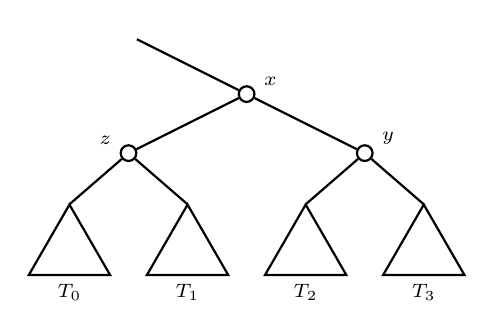
\begin{tikzpicture}
[-,thick,%
  lineDecorate/.style={-,thick},%
  nodeDecorate/.style={shape=regular polygon,regular polygon sides=3,inner sep=6pt,draw,thick},%
scale=0.5]
\scriptsize
%% nodes and edges
\node at (0,0) {}
  [sibling distance=6cm]
  child[missing]
  child {node[shape=circle,inner sep=2pt,draw] (x) {}
    child {node[shape=circle,inner sep=2pt,draw] (z) {}}
    child {node[shape=circle,inner sep=2pt,draw] (y) {}}
  };
%% node labels
\node[above left] at (z.west) {$z$};
\node[above right] at (y.east) {$y$};
\node[above right] at (x.east) {$x$};
%% generic trees and their labels
\foreach \nodename/\x/\y/\direction/\navigate in {
  T_0/-1.5/-5.5/below/south, T_1/1.5/-5.5/below/south,
  T_2/4.5/-5.5/below/south, T_3/7.5/-5.5/below/south}
{
  \node[nodeDecorate] (\nodename) at (\x,\y) {};
  \node [\direction] at (\nodename.\navigate) {$\nodename$};
}
%% connect nodes to generic trees
\path
(z) edge[lineDecorate] node {} (-1.5,-4.3)
(z) edge[lineDecorate] node {} (1.5,-4.3)
(y) edge[lineDecorate] node {} (4.5,-4.3)
(y) edge[lineDecorate] node {} (7.5,-4.3);
\end{tikzpicture}
}
%%
%%
\subfigure[Double rotation: left rotation of $x$ over $y$, then right
rotation over $z$.]{
\label{fig:tree_data_structures:AVL_trinode_restructure:left_right_rotate}
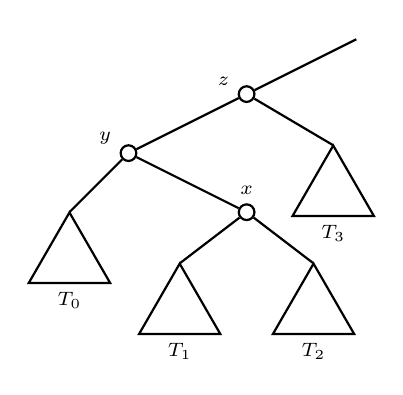
\begin{tikzpicture}
[-,thick,%
  lineDecorate/.style={-,thick},%
  nodeDecorate/.style={shape=regular polygon,regular polygon sides=3,inner sep=6pt,draw,thick},%
scale=0.5]
\scriptsize
%% nodes and edges
\node at (0,0) {}
  [sibling distance=6cm]
  child {node[shape=circle,inner sep=2pt,draw] (z) {}
    child {node[shape=circle,inner sep=2pt,draw] (y) {}
      child[missing]
      child {node[shape=circle,inner sep=2pt,draw] (x) {}}
    }
    child[missing]
  }
  child[missing];
%% node labels
\node[above left] at (z.west) {$z$};
\node[above left] at (y.west) {$y$};
\node[above] at (x.north) {$x$};
%% generic trees and their labels
\foreach \nodename/\x/\y/\direction/\navigate in {
  T_0/-7.5/-5.7/below/south, T_1/-4.7/-7/below/south,
  T_2/-1.3/-7/below/south, T_3/-0.8/-4/below/south}
{
  \node[nodeDecorate] (\nodename) at (\x,\y) {};
  \node [\direction] at (\nodename.\navigate) {$\nodename$};
}
%% connect nodes to generic trees
\path
(y) edge[lineDecorate] node {} (-7.5,-4.5)
(x) edge[lineDecorate] node {} (-4.7,-5.8)
(x) edge[lineDecorate] node {} (-1.3,-5.8)
(z) edge[lineDecorate] node {} (-0.8,-2.8);
\end{tikzpicture}
%%
%%
\qquad\qquad
%%
%%
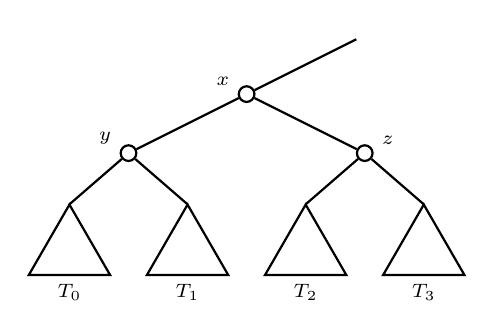
\begin{tikzpicture}
[-,thick,%
  lineDecorate/.style={-,thick},%
  nodeDecorate/.style={shape=regular polygon,regular polygon sides=3,inner sep=6pt,draw,thick},%
scale=0.5]
\scriptsize
%% nodes and edges
\node at (0,0) {}
  [sibling distance=6cm]
  child {node[shape=circle,inner sep=2pt,draw] (x) {}
    child {node[shape=circle,inner sep=2pt,draw] (y) {}}
    child {node[shape=circle,inner sep=2pt,draw] (z) {}}
  }
  child[missing];
%% node labels
\node[above right] at (z.east) {$z$};
\node[above left] at (y.west) {$y$};
\node[above left] at (x.west) {$x$};
%% generic trees and their labels
\foreach \nodename/\x/\y/\direction/\navigate in {
  T_0/-7.5/-5.5/below/south, T_1/-4.5/-5.5/below/south,
  T_2/-1.5/-5.5/below/south, T_3/1.5/-5.5/below/south}
{
  \node[nodeDecorate] (\nodename) at (\x,\y) {};
  \node [\direction] at (\nodename.\navigate) {$\nodename$};
}
%% connect nodes to generic trees
\path
(y) edge[lineDecorate] node {} (-7.5,-4.3)
(y) edge[lineDecorate] node {} (-4.5,-4.3)
(z) edge[lineDecorate] node {} (-1.5,-4.3)
(z) edge[lineDecorate] node {} (1.5,-4.3);
\end{tikzpicture}
}
\end{figure}

\end{document}
